\begin{frame}[plain]{Main Functions}
	% this is a comment
\pause
\begin{itemize}
\item Function: Speed control of the car	
\pause
	\begin{itemize}
	\item<1-> Input: distance from objects ahead from the ultrasound sensor
	\pause
	\item<2-> Communication protocol: Uart communication
	\pause
	\item<3-> Output: Duty cycle for the motor
	\end{itemize}
\end{itemize}
\pause

Note: Time delay after each iteration to prevent ultrasound sensors from crashing

\vspace{1cm}
	
\pause
\begin{itemize}
\item Function: Car steering to follow the line	
\pause
	\begin{itemize}
	\item<1-> Input: camere input (using Raspberry Pi)
	\pause
	\item<2-> Communication protocol: Uart communication
	\pause
	\item<3-> Output: Duty cycle for the servomotor 
	\end{itemize}
\end{itemize}
\pause
Note: Disable bluetooth on Raspberry Pi 3 in order for Uart communication to work
	%\pause
	%\\
	%Note: Disable bluetooth on Raspberry Pi 3 in order for Uart communication to work 
	%\begin{figure}
	%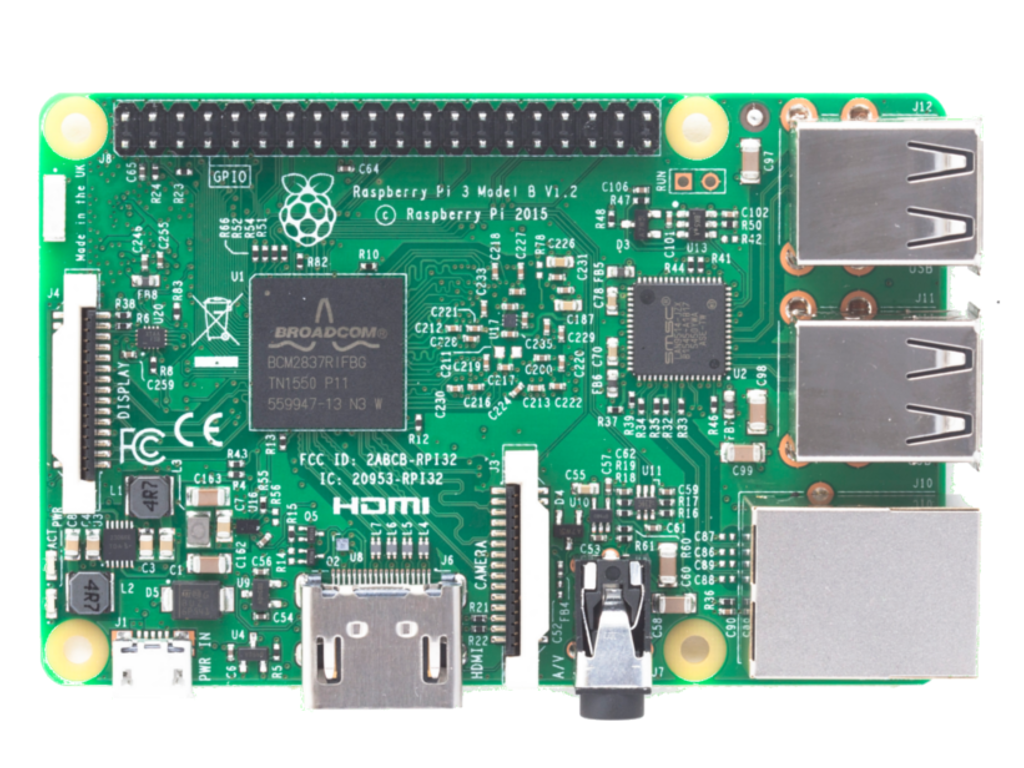
\includegraphics[width=7cm, height=5cm]{raspi2.png}
	%\end{figure}
	
	%\vspace{2cm}
	
\end{frame}

\begin{frame}[plain]{Adaptive Cruise Control}

What is Adaptive Cruise Control?
\pause
\begin{itemize}
	\item Automotive safety feature that allows the vehicle to adapt its speed to the traffic environment 
	\pause
	\item In real cars, a long range radar sensor is used to detect the cars, here we use an ultrasound sensor
\end{itemize}
\pause	
\vspace{1cm}
ACC Algorithm
\pause
\begin{itemize}
	\item if distance from ultrasound sensor $\leq$ a minimum set distance ($distance_{min}$) --> stop
	\pause
	\item if distance from ultrasound sensor $\geq$ a maximum set distance ($distance_{max}$) --> drive with maximum speed
	\pause
	\item else (distance lies within $distance_{min}$ and $distance_{max}$) --> adapt speed according to distance:
	\pause
	$$Current Speed = Maximum Speed * \frac{distance}{distance_{max}}$$
\end{itemize}
\end{frame}

\begin{frame}[plain]{Adaptive Cruise Control}
 \includemedia[
    width=0.4\linewidth,
    height=0.3\linewidth,
    label='firsttry',
    %addresource="C:/_Book/_Website/40631-H.264.mp4",
    activate=pageopen,
   %flashvars={source="C:/_Book/_Website/40631-H.264.mp4"}
  ]{}{ACC.mp4}
The video should appear just above.
%    \flashmovie{Wildlife.wmv}
	
\end{frame}

\begin{frame}[plain]{Main Code}
The main code runs as follows:
\begin{enumerate}
\item Receive distance from ultrasound sensor 
\pause
\item Receive driving angle from Raspberry Pi
\pause
\item Calculate driving speed according to the adaptive cruise control algorithm
\pause
\item Calculate the servomotor's duty cycle to follow the line
\pause
\item Time delay to prevent ultrasound sensor from crashing
\pause
\item Repeat ..
\end{enumerate}
\end{frame}